%!TEX root = ..\MainFile.tex
\section{Результаты выполнения работы} % (fold)
\label{sec:WorkResults}	
    \subsection{Особенности разработанной программы} % (fold)
    \label{sub:ProgrammFetures}
        
    % subsection ProgrammFetures (end)

    \subsection{Результаты полученные при симуляции} % (fold)
    \label{sub:ProgrammResults}
        Как показала практика, надежды уменьшить число шагов при помощи алгоритма, представленного на рис. [] не оправдались, поскольку среднее число шагов, необходимое для достижения стабильного распределения скоростей по высоте оказалось порядка $6 \times 10^5$ С другой стороны, можно уверенно говорить что значения скорости снимались в достаточно стабильном состоянии.

        Проведенная проверка показала, что результаты, получаемые при использовании чисел одинарной и двойной точности совпадают в пределах погрешности. (см. рис []), при этом использование чисел одинарной точности увеличивает скорость вычислений примерно в три раза, и позволяет достичь пиковой производительности в 3.5 ТFlops.

        Побочным результатом, позволяющим судить о правильной работе программы является соответствие кривых, полученных при запуске в стандартном режиме (т.е. режиме модели Вичека), с кривыми полученными другими исследователями, например, в работе \cite{vicsek1995}.

        Главный результат работы заключается в том, что полученные профили скоростей однозначно свидетельствуют об отсутствии трения как внутри жидкости самодвижущихся частиц, так и при взаимодействии частиц со стенками. 

        \begin{figure}
        \centering
        \begin{subfigure}{0.45\textwidth}
                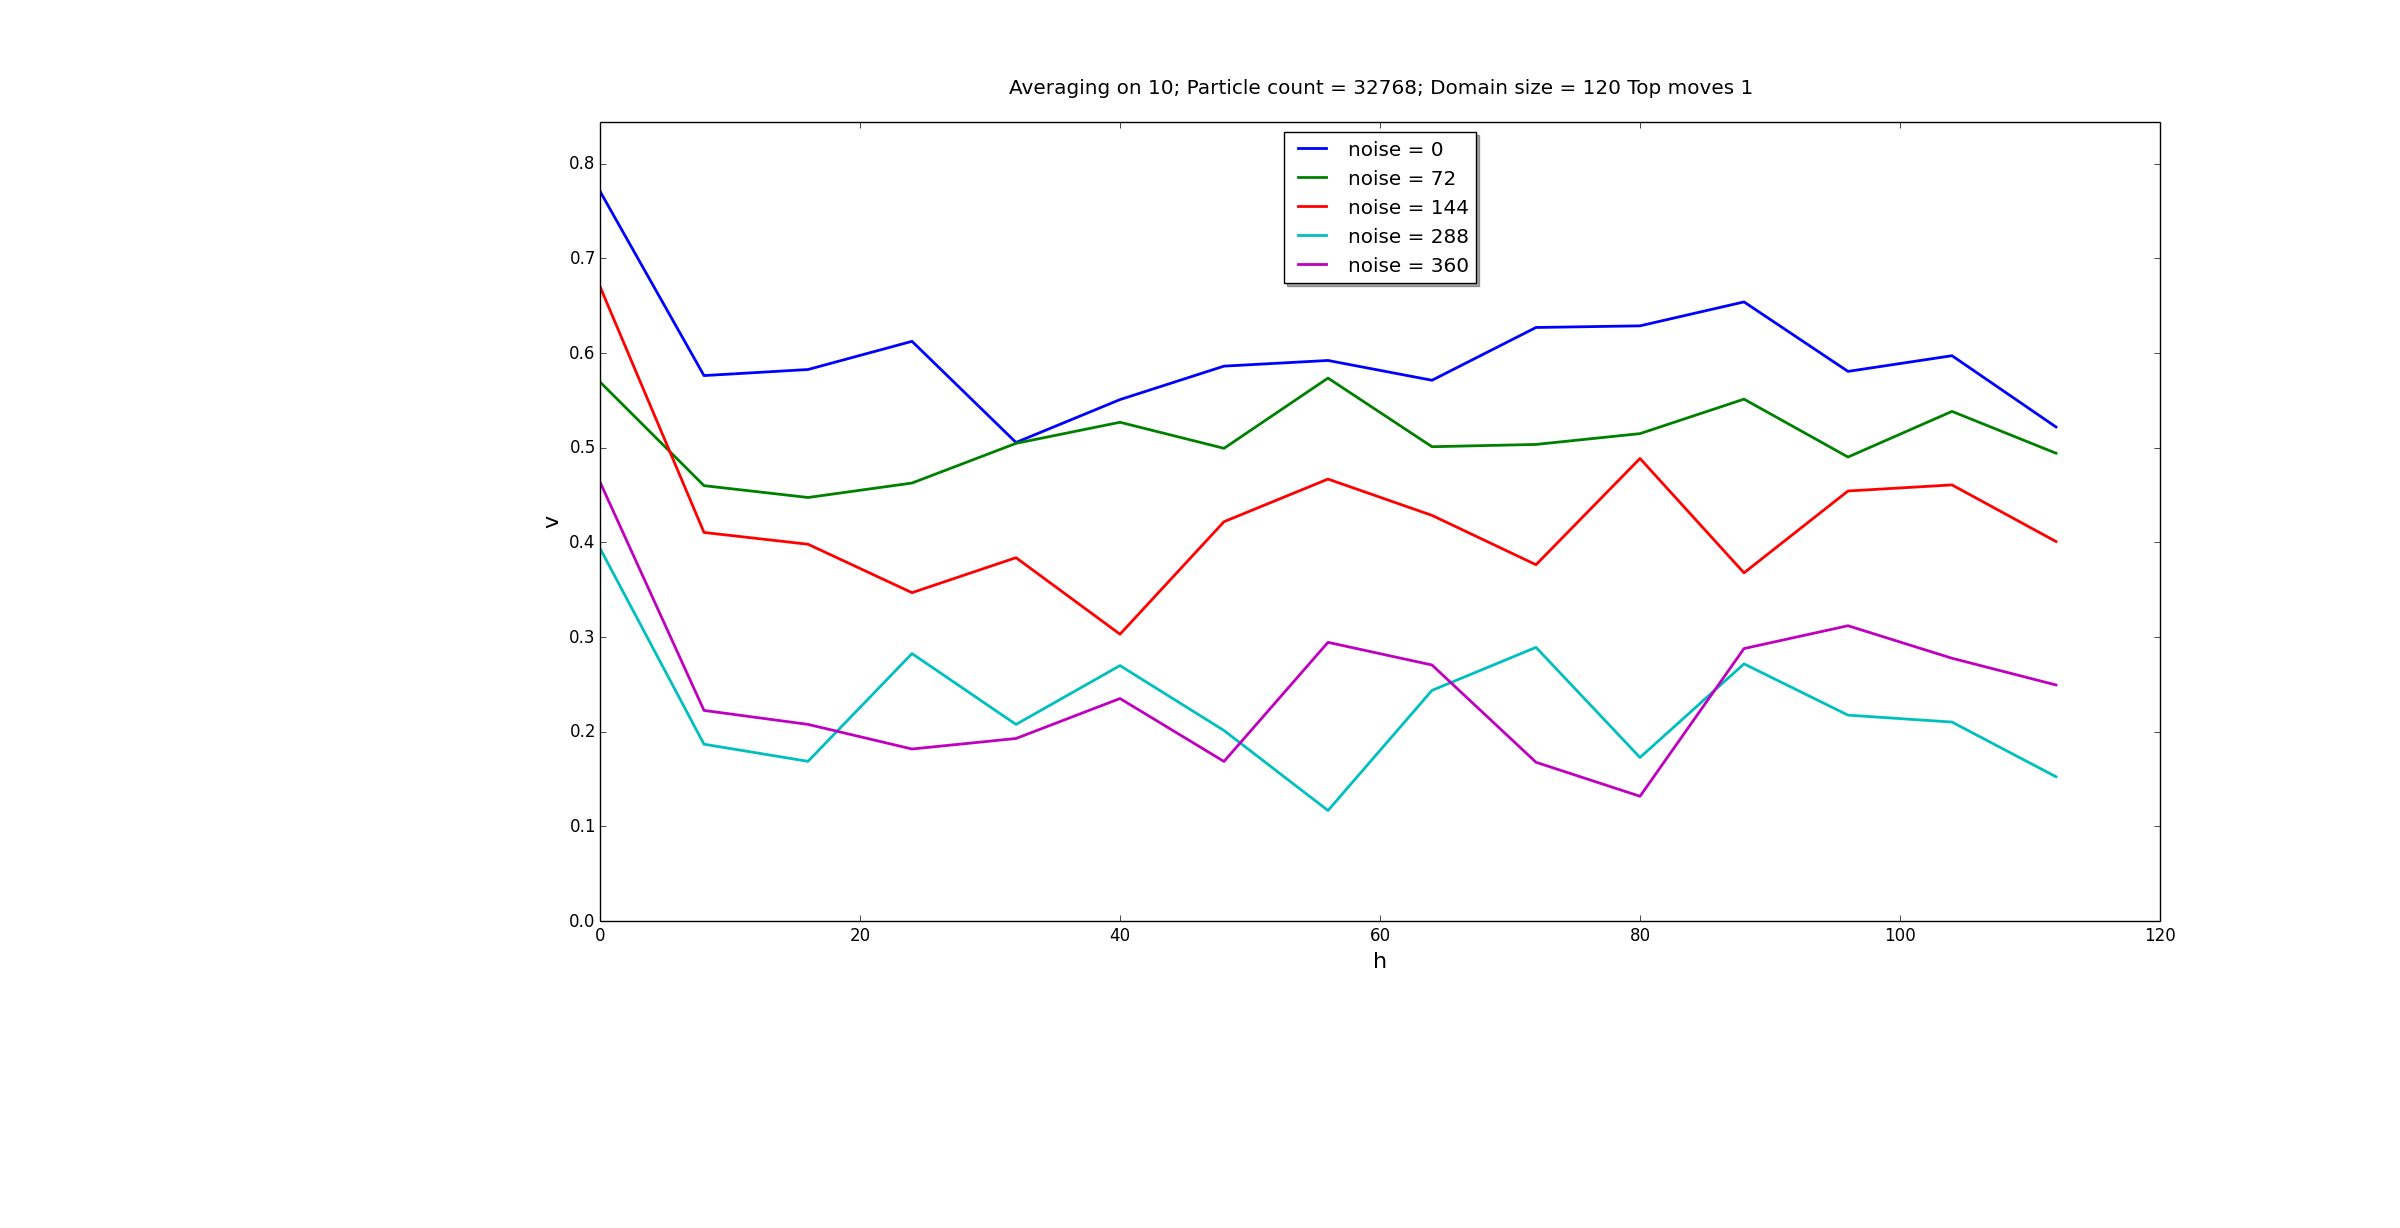
\includegraphics[width=\textwidth]{32k_slices}
                \caption{Профили для 32000}
                \label{fig:Results:32k}
        \end{subfigure}
        \begin{subfigure}{0.45\textwidth}
                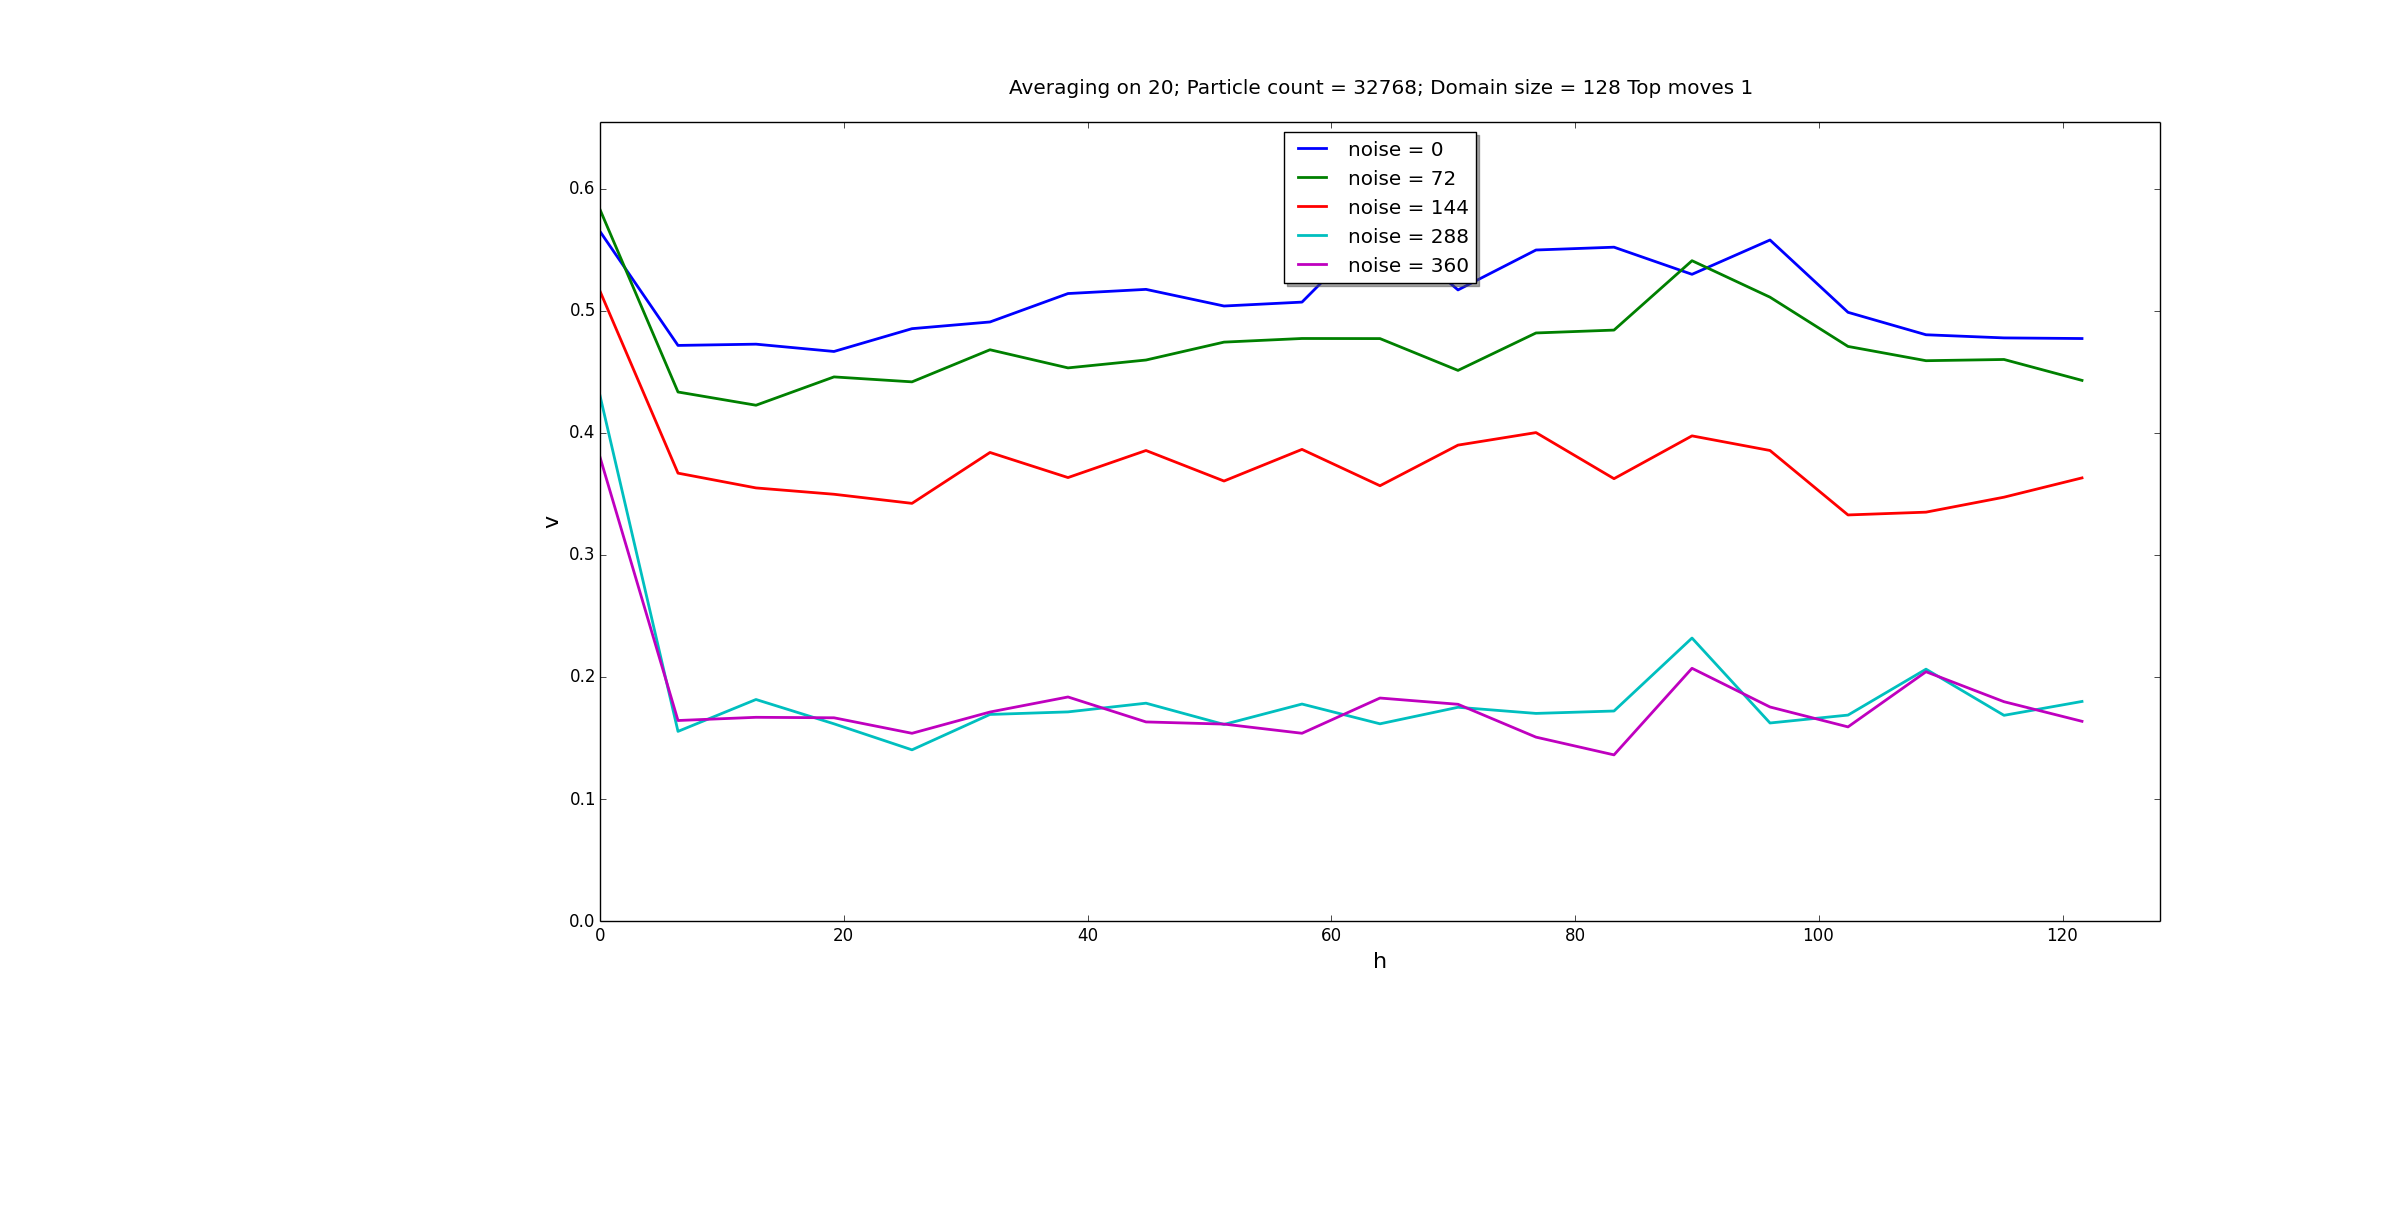
\includegraphics[width=\textwidth]{32k_slicesOldAlg}
                \caption{профили для 32000, оценивая уравшовешенность по средней скорости}
                \label{fig:Results:32kOld}
        \end{subfigure}
        \begin{subfigure}{0.45\textwidth}
                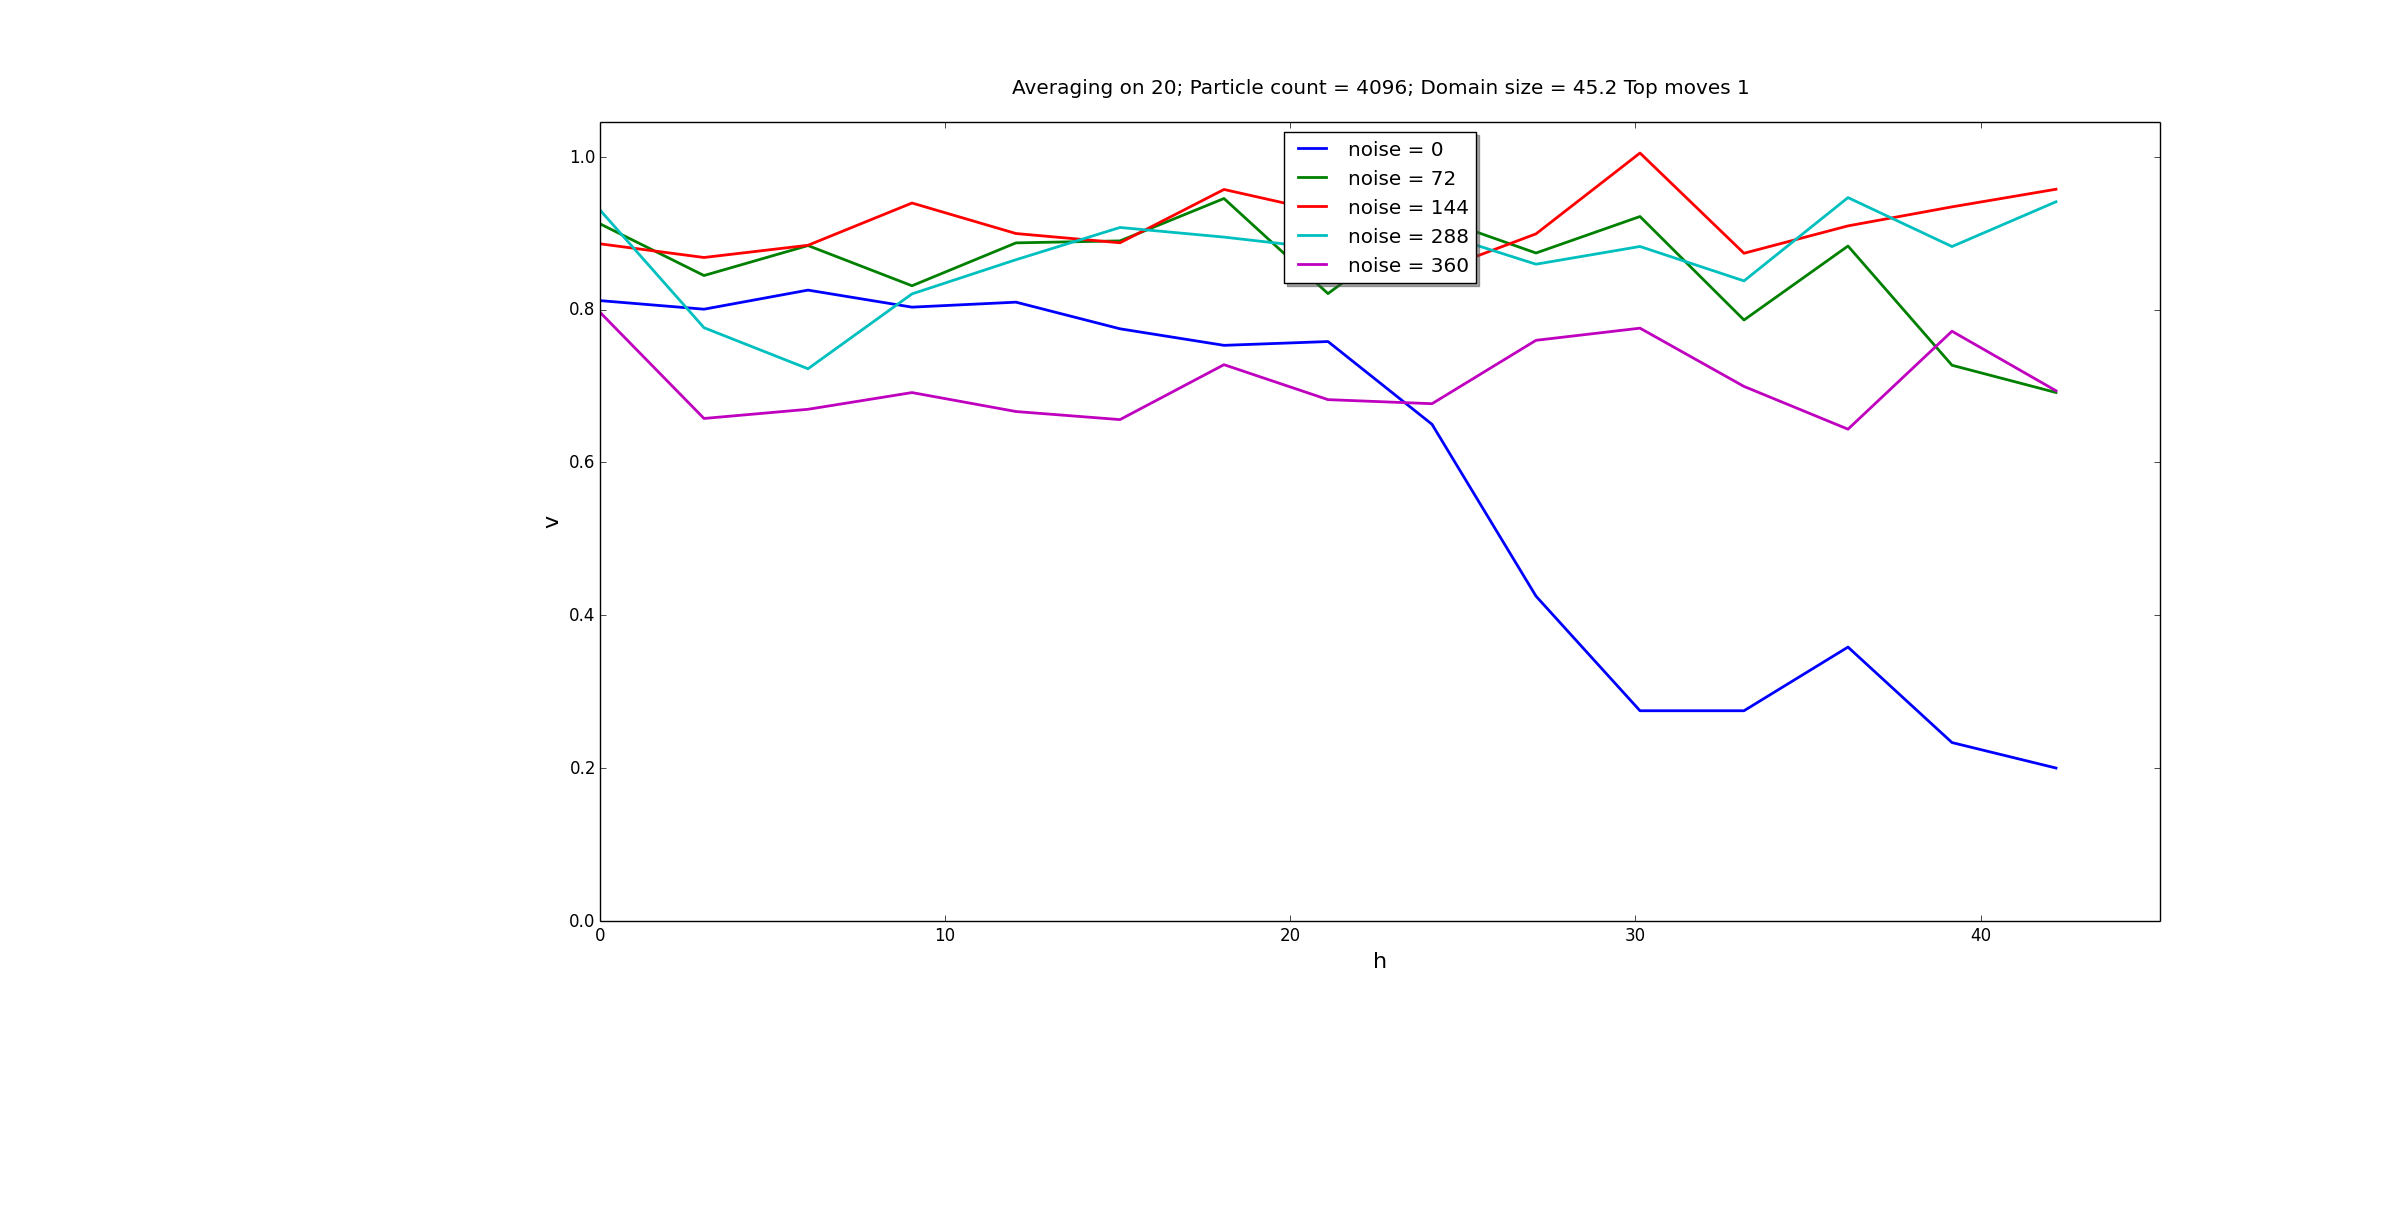
\includegraphics[width=\textwidth]{4k_slices_newAlg}
                \caption{профили для 4000}
                \label{fig:Results:4kNew}
        \end{subfigure}
        \begin{subfigure}{0.45\textwidth}
                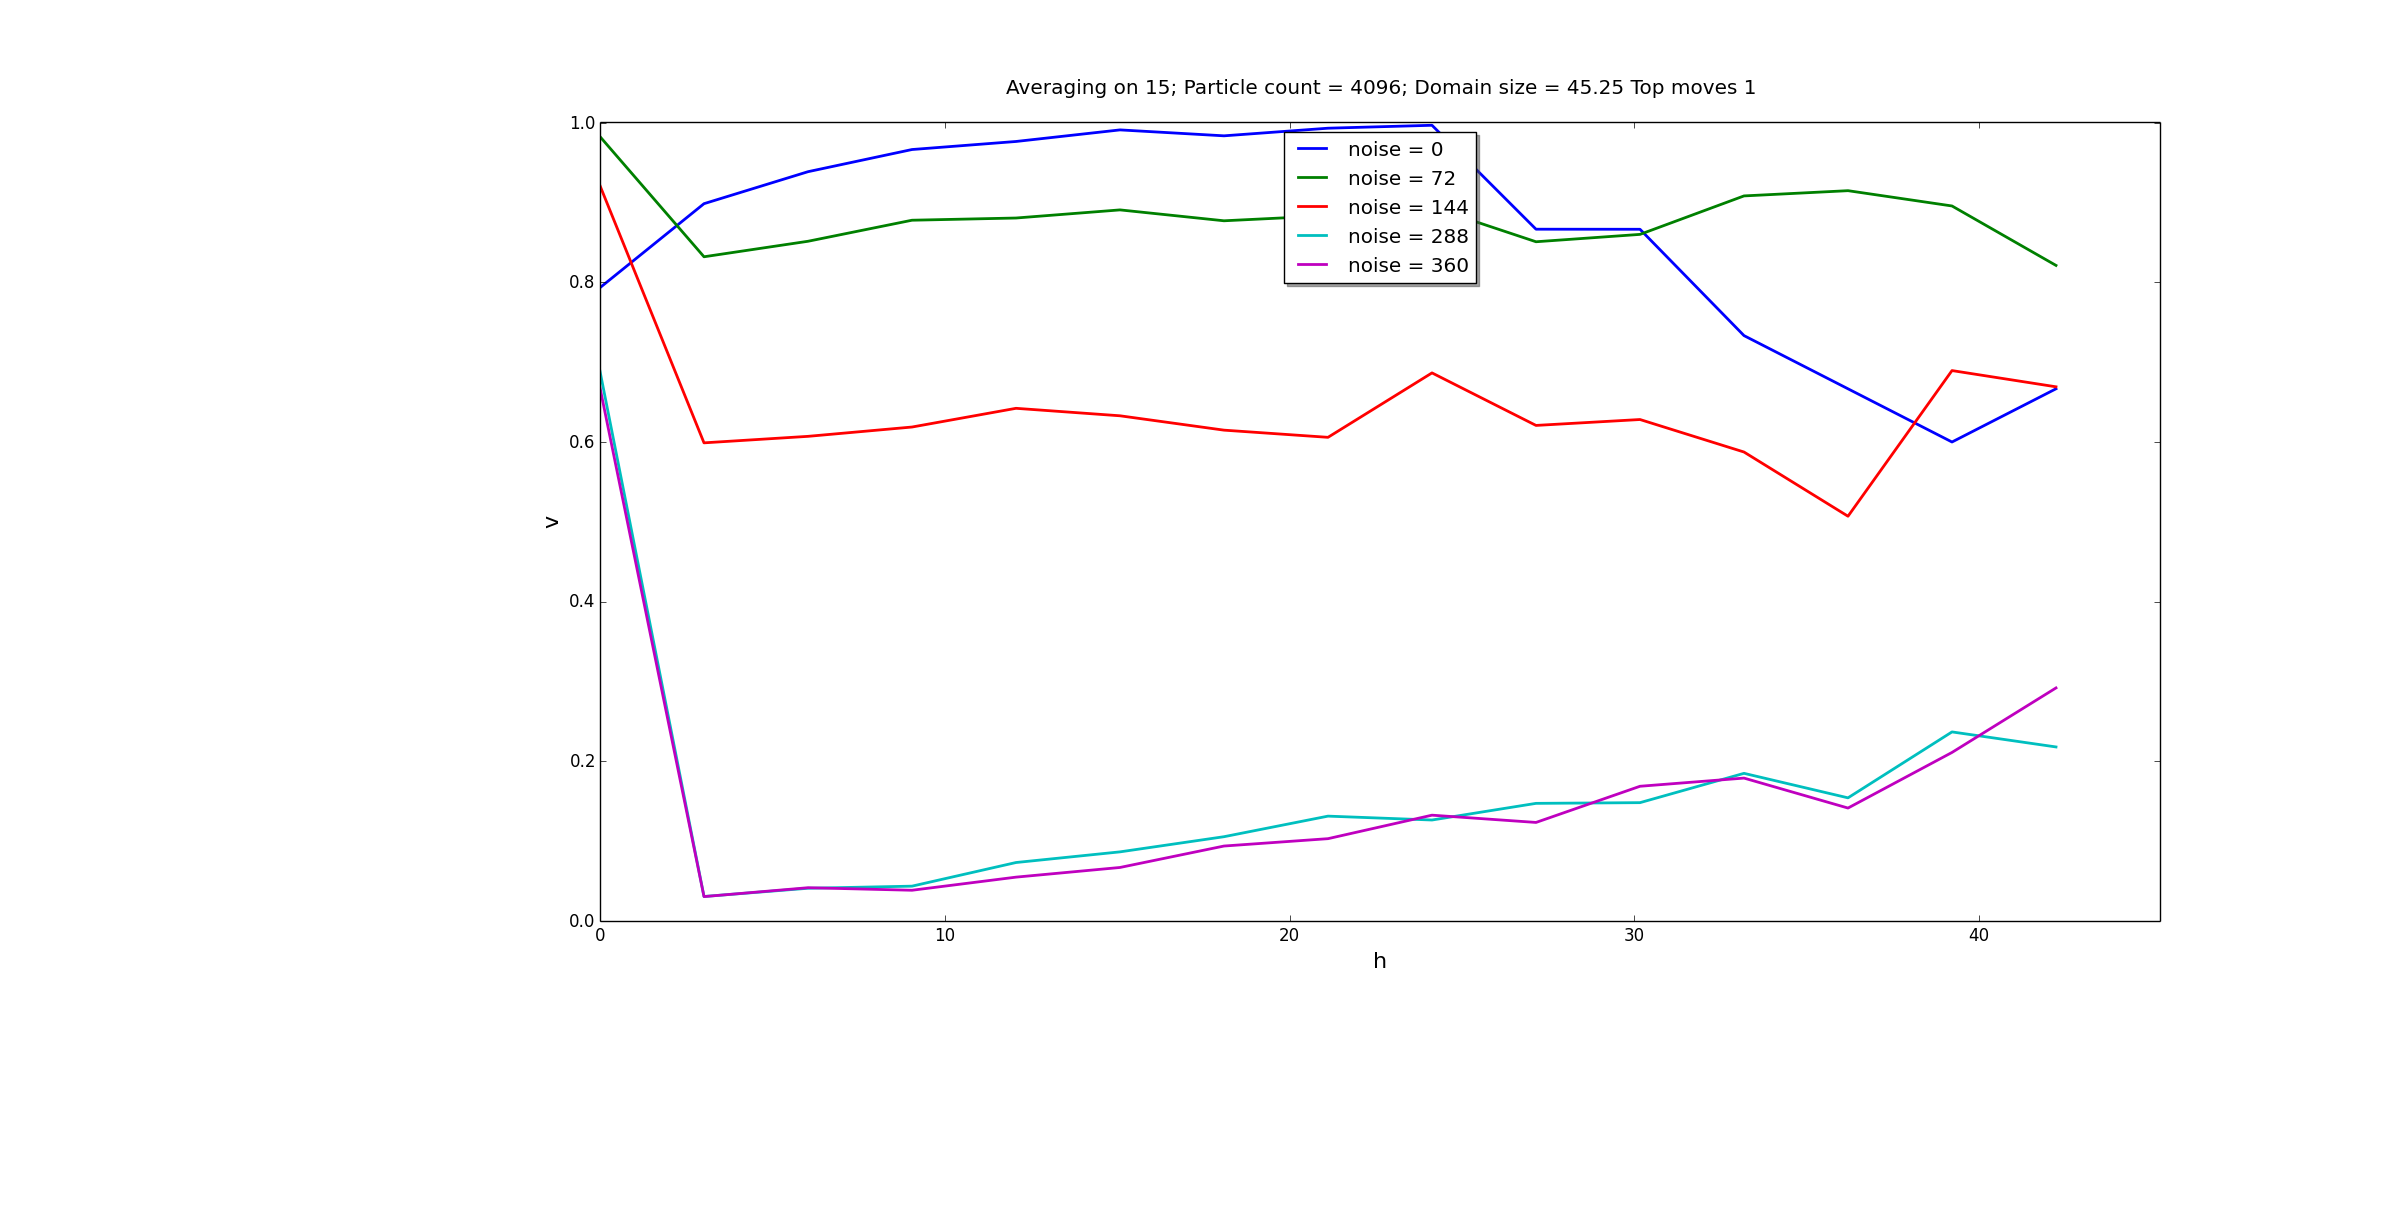
\includegraphics[width=\textwidth]{4k_slices_oldAlg}
                \caption{профили для 4000, оценивая уравшовешенность по средней скорости}
                \label{fig:Results:4kOld}
        \end{subfigure}
        \caption{Профили скоростей течения Куэтта}
        \label{fig:Results}
        \end{figure}

        Рассматривая графики, представленные на рис. \ref{fig:Results}, можно сделать несколько наблюдений.
        \begin{enumerate}
            \item Для высоких значений шума (выше фазового перехода) профиль скорости достаточно прямой, и скорость оказывается невысока
            \item При уменьшении шума до значений существенно ниже знаений фазового перехода, профиль сохраняет прямую геометрию, при том что средняя скорость увеличивается.
            \item Только при значениях шума ниже 72, начинает проявляться профиль, подобный стандартному для Куэттовского потока.
        \end{enumerate}

        Из вышеприведенных наблюдений следуют совершенно прямолинейные выводы.



        \begin{itemize}
            \item Во-первых, при высоких значениях шума вязкостью среды можно пренебречь.
            \item Во-вторых, при низких значениях шума поведение жидкости отличается от такового при высоких значениях шума, что требует дальнейшего рассмотрения. \marginpar{Низкошумовой предел}
        \end{itemize}

        Кроме того, хотелось бы обратить внимание на следующий факт: при использовании средней скорости как критерия стабильности состояния, влияние граничого слоя оказывается намного выше из-за того что система не успевает релаксировать. Это приводит к повышенным значениям скорости у границ. И если для верхней границы причина этого очевидна, то для нижней это может быть обьяснено тем, что при взаимодействии отраженных и набегающих частиц средняя скорость оказывается направлена вдоль границы. (см. рис []) Поскольку симметрия задачи нарушена верхней стенкой, то преимущественным оказывается направление совпадающее с направлением верхней стенки, что и приводит к увеличению средней скорости в нижней области.
    % subsection ProgrammResults (end)
% section WorkResults (end)	